\subsection{}
Where does the demand curve come from?
\begin{definition}
    \emph{Utility} loosely is the happiness or satisfaction you get from a good.\\
    It is measured in \emph{utils}. The first good you consume gives you the most utility.
    Each additional good gives you less utility. Each good provides a \emph{Marginal Utility}, 
    which is the additional utility you get from consuming one more good. \emph{Diminishing Marginal Utility} 
    is the idea that the more you consume, the less utility you get from each additional good.
\end{definition}
\begin{definition}
    \emph{Total Utility} is the consumer's total satisfaction resulting from the consumption of a given product.
\end{definition}
\begin{definition}
    \emph{Marginal Utility} is the additional satisfaction obtained from consuming one additional unit of a product.
\end{definition}
\begin{definition}
    \emph{Diminishing Marginal Utility}, the utility that any consumer derives from successive units of a particular product consumed
    over some period of time diminishes as total consumption of the product increases.
\end{definition}

\begin{figure}[H]
    \centering
    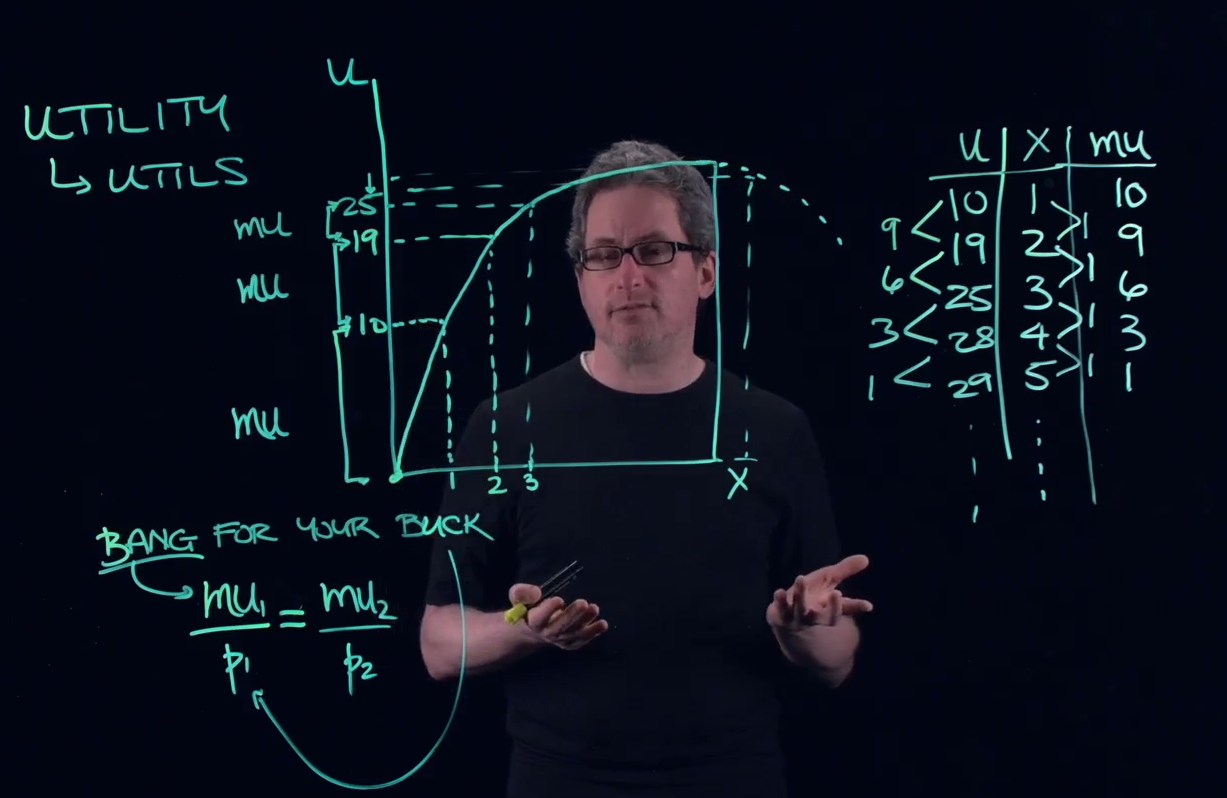
\includegraphics[width=0.5\textwidth]{Chapter6/Utility.png}
    \caption{Utility}
    \label{fig:Utility}
\end{figure}
What if we compare the utility of different goods?\\
We need to factor in the utility and costs.
\begin{equation}
    \begin{gathered}
        \frac{\text{mu}_1}{P_1} > \frac{\text{mu}_2}{P_2}\\
        \frac{\text{mu}_1}{\text{mu}_2} > \frac{P_1}{P_2}\\
        \frac{\text{mu}_1}{\text{mu}_2} = \text{mrs (marginal rate of substitution, how much willing for 1 more good 1)}\\
        \frac{P_1}{P_2} = \text{Relative price ratio (How much you have to give up for 1 more good 1)}\\
        \text{If mrs} > \text{Relative price ratio, you are willing to give up good 2.}\\
        \text{If mrs = Relative price ratio, you are indifferent.}
    \end{gathered}
\end{equation}
After enough transactions the inequality may change.\\
A consumer wants to equalize the equation.
\par
The market demand curve is the sum of all individual demand curves.
\begin{figure}[H]
    \centering
    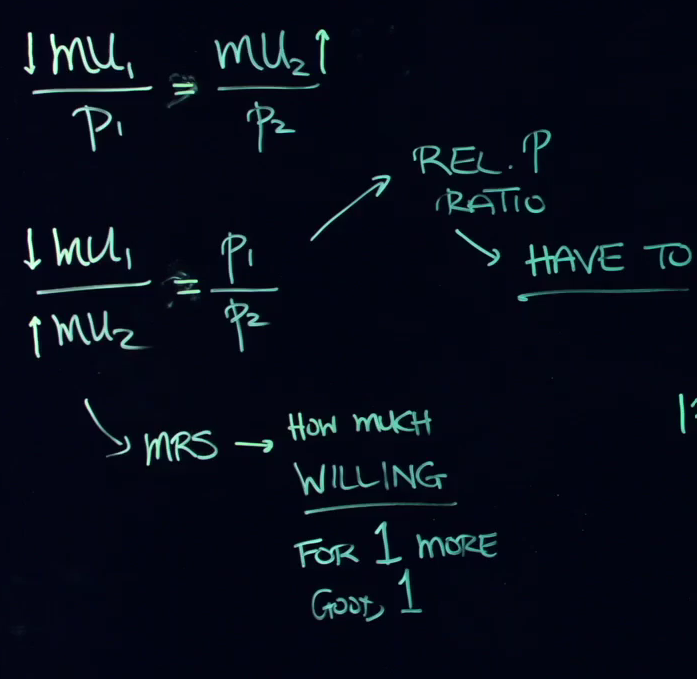
\includegraphics[width=0.5\textwidth]{Chapter6/MarginalUtility.png}
    \caption{Marginal rate of substitution}
    \label{fig:Marginal_rate_of_substitution}
\end{figure}
\par
We assume all consumers are rational and acting in self-interest. Some economists think consumers may be irrational but maybe some consumers are overwhelmed by choice,
or the information is presented in different ways.